\documentclass[leqno]{article}
% Shared QBT/Soln pack preamble for resources.danieljsmith.org.
\usepackage{graphicx}
\usepackage{dsfont}
\usepackage{mathtools}
\usepackage{amssymb}
\usepackage{amsmath}
\usepackage{mleftright}
\usepackage{amsthm}
\usepackage{float}
\usepackage{ragged2e}
\usepackage{tensor}
\usepackage{fancyhdr}
\usepackage{empheq}
\usepackage[most]{tcolorbox}
\usepackage{enumitem}
\usepackage{dirtytalk}
\usepackage{marginnote}
\usepackage{microtype}
\usepackage[
  a4paper,
  left=0.8in,
  right=1in,
  top=1in,
  bottom=0.5in,
  headheight=14pt,
  headsep=0.4in
]{geometry}
\setlength{\parindent}{0cm}

% TikZ / PGFPlots
\usepackage{pgfplots}
\pgfplotsset{compat=1.18}
\usepgfplotslibrary{fillbetween, polar}
\usetikzlibrary{calc, positioning}
\usetikzlibrary{angles, quotes}
\usetikzlibrary{arrows.meta}
\usetikzlibrary{decorations.pathreplacing, decorations.markings}
\usetikzlibrary{patterns}
\usetikzlibrary{intersections}

% Links and contents. The contents follow the TMUA papers: compact entries,
% no dot leaders, and each question's mark total in grey after its label.
\usepackage{tocloft}
\tocloftpagestyle{fancy}
\setlength{\cftbeforesubsecskip}{2pt}
\setlength{\cftsubsecindent}{1.5em}
\setlength{\cftsubsecnumwidth}{0pt}
\renewcommand{\cftsubsecfont}{\small\color{black}}
\renewcommand{\cftsubsecpagefont}{\small\color{black}}
\renewcommand{\cftsubsecleader}{\hfill}
\usepackage[colorlinks=true,linkcolor=black,citecolor=magenta,urlcolor=black]{hyperref}%
\urlstyle{same}

% Pack macros
% \marks also adds its value to the current question's total in the .aux
% file, so the contents show each total from the second pass. The write
% happens at shipout, so a box typeset more than once counts once. The
% pack's mark total for the contents-page title is summed the same way.
\makeatletter
\newcount\djs@totalmarks
\newcommand{\djsAddMarks}[2]{%
  \global\advance\djs@totalmarks#2\relax
  \@ifundefined{djs@marks@#1}%
    {\expandafter\xdef\csname djs@marks@#1\endcsname{#2}}%
    {\expandafter\xdef\csname djs@marks@#1\endcsname
      {\the\numexpr\csname djs@marks@#1\endcsname+#2\relax}}}
\RenewDocumentCommand{\marks}{o m}{%
  \protected@write\@auxout{}{\string\djsAddMarks{\number\value{enumi}}{#2}}%
  \IfValueTF{#1}%
    {\marginnote{\raggedright\textbf{[#2]}}[#1]}%
    {\marginnote{\raggedright\textbf{[#2]}}}%
}
\makeatother

\newcommand{\vspacerule}[2]{%
  \par\vspace*{#1}%
  \noindent\hrulefill\par
  \vspace*{#2}%
}

\definecolor{scarlet}{RGB}{205, 40, 75}
% Site colours for the contents-page title: the accent, the rule colour, a
% stronger rule colour for the path separator, and the muted text colour.
\definecolor{djsBurgundy}{RGB}{118, 59, 67}
\definecolor{djsHairline}{RGB}{216, 213, 205}
\definecolor{djsSlash}{RGB}{170, 166, 158}
\definecolor{djsMuted}{RGB}{96, 101, 106}

% Worked-solution box, adapted from the TMUA worked-solutions box. A white breakable box with a left scarlet rule and no surrounding
% frame or tint. A part that breaks fills the rest of its page, so the rule
% runs to the bottom margin; the unbroken or last part ends in a short
% horizontal foot rule so a solution visibly stops. Unlike the TMUA box there
% is no answer label. The box does not grow to the left, so the rule sits at
% the text edge; growing to the right keeps the usable line width close to the
% old tcolorbox Solution box.
% Spacing inside the box: paragraphs are 6pt apart, so source blank lines show
% (solutions put one after each display and none between a lead-in and its
% display). Every display gets 6pt above and 10pt below, whatever the length
% of its lead-in line; align rows are spread by an 8pt \jot; solution parts
% are 14pt apart and sub-parts 8pt; \left and \right space like ordinary
% brackets (mleftright); no single line is stranded at a page break; and
% neither the Solution label nor the line before a list ends a page. No
% skip can shrink, so full pages are not squeezed.
\newtcolorbox{djsSolution}{%
  enhanced, breakable, frame hidden, sharp corners, colback=white,
  height fixed for=first and middle, height fill,
  extras unbroken and last={natural height},
  borderline west={2.2pt}{0pt}{scarlet},
  left=11pt, right=0pt, top=5pt, bottom=13pt,
  before skip=13pt, after skip=4pt,
  grow to right by=10mm,
  overlay unbroken and last={%
    \fill[scarlet] (frame.south west)
      rectangle ([xshift=3.5cm, yshift=2.2pt]frame.south west);},
  before upper={{\color{scarlet}\bfseries Solution}\par\nobreak\vspace{4pt}%
    \setlength{\parskip}{6pt plus 2pt}%
    \setlength{\abovedisplayskip}{6pt plus 2pt}%
    \setlength{\abovedisplayshortskip}{6pt plus 2pt}%
    \setlength{\belowdisplayskip}{10pt plus 2pt}%
    \setlength{\belowdisplayshortskip}{10pt plus 2pt}%
    \setlength{\jot}{8pt}%
    \setlist{parsep=6pt plus 2pt, topsep=6pt plus 2pt, beginpenalty=10000}%
    \setlist[enumerate,1]{itemsep=14pt plus 2pt}%
    \setlist[enumerate,2]{itemsep=8pt plus 2pt}%
    \mleftright
    \clubpenalty=10000 \widowpenalty=10000 \displaywidowpenalty=10000\relax}}

% Optional smaller figure inside a solution box. \scalebox shrinks node text
% with the drawing. Not applied to existing figures.
\newcommand{\SolnFigureScale}{0.85}
\newsavebox{\djsSolnFigureBox}
\newenvironment{djsSolutionFigure}
  {\par\vspace{4pt}\begin{center}\begin{lrbox}{\djsSolnFigureBox}}
  {\end{lrbox}\scalebox{\SolnFigureScale}{\usebox{\djsSolnFigureBox}}%
   \end{center}\vspace{2pt}\par}

\newcommand{\cxl}[2]{%
  \tikz[baseline=(X.base)]{%
    \node[inner sep=0pt, outer sep=0pt, text=#1] (X) {$#2$};
    \draw[#1, line width=0.4pt] (X.south west)--(X.north east);
  }%
}

% Page-style hook run at the contents page and each question's opening page.
% A no-op for QBT packs; \djsSolnHeader points it at the fancy header.
\newcommand{\djsQuestionPageStyle}{}

% A contents entry: "Question N" in a box wide enough for two digits, so the
% mark totals line up, then the total in grey. Bookmarks keep "Question N".
\makeatletter
\newlength{\djsTocLabelWidth}
\newcommand{\djsTocMarks}[1]{%
  \@ifundefined{djs@marks@#1}{}{%
    {\footnotesize\itshape\color{black!45}%
     \csname djs@marks@#1\endcsname~mark%
     \ifnum\csname djs@marks@#1\endcsname=1 \else s\fi}}}
\newcommand{\djsTocEntry}[1]{%
  \texorpdfstring
    {\settowidth{\djsTocLabelWidth}{Question 00}%
     \makebox[\dimexpr\djsTocLabelWidth+0.9em\relax][l]{Question #1}%
     \djsTocMarks{#1}}%
    {Question #1}}
\makeatother

% The question count for the contents-page title is written to the .aux at
% the end of the document, so it also appears from the second pass.
\newcounter{djsQuestions}
\newcommand{\questionitem}{%
  \djsQuestionPageStyle
  \item\phantomsection
  \stepcounter{djsQuestions}%
  \addcontentsline{toc}{subsection}{\protect\djsTocEntry{\number\value{enumi}}}%
}
\makeatletter
\newcommand{\djsSetQuestionCount}[1]{\gdef\djs@questioncount{#1}}
\AtEndDocument{\immediate\write\@auxout
  {\string\djsSetQuestionCount{\number\value{djsQuestions}}}}
\makeatother

\renewcommand{\contentsname}{Questions}

% \djsPackHeader[<link content tag>]{<left header>}; the tag says which
% document a click on the header link came from.
\newcommand{\djsPackHeader}[2][questions]{%
  \pagestyle{fancy}%
  \fancyhead{}%
  \fancyfoot{}%
  \renewcommand{\headrulewidth}{0.9pt}%
  \lhead{#2}%
  \chead{}%
  \rhead{\href{https://danieljsmith.org/?utm_source=pdf&utm_campaign=further-maths&utm_content=#1}{danieljsmith.org}}%
}

% The header's topic is also the contents-page title, under which a label
% says which booklet this is.
\newcommand{\djsPackTitle}{}
\newcommand{\djsBookletLabel}{}
\newcommand{\djsQbtHeader}[1]{%
  \djsPackHeader{#1}%
  \renewcommand{\djsPackTitle}{#1}%
  \renewcommand{\djsBookletLabel}{Questions by topic}%
}

% The colophon at the foot of page one, independent of the page style: the
% contents-page title's hairline led by a short scarlet rule, then the date on
% the left and a link to the site on the right, all inside the bottom margin.
% Its sizes are fixed, so it matches the TMUA papers' colophon. The document
% supplies the date; recompiling never changes it.
\makeatletter
\newcommand{\djsLastUpdated}[1]{%
  \AtBeginDocument{\AddToHookNext{shipout/foreground}{\djs@colophon{#1}}}}
\newcommand{\djs@colophon}[1]{%
  \put(0.8in,-\dimexpr\paperheight-0.47in\relax){%
    \makebox[0pt][l]{\color{djsHairline}%
      \rule[0.9pt]{\dimexpr\paperwidth-1.8in\relax}{0.6pt}}%
    \makebox[0pt][l]{\color{scarlet}\rule{3.5cm}{2.2pt}}}%
  \put(0.8in,-\dimexpr\paperheight-0.32in\relax){\makebox[0pt][l]{%
    \fontsize{9}{11}\selectfont Last updated #1}}%
  \put(\dimexpr\paperwidth-1in\relax,-\dimexpr\paperheight-0.32in\relax){%
    \makebox[0pt][r]{\fontsize{7}{8.5}\selectfont\color{djsMuted}%
      Latest version at \href{https://resources.danieljsmith.org/}%
        {\color{black}resources.danieljsmith.org}}}}
\makeatother

% Solutions packs show the header only on the contents page and each
% question's opening page, so it never appears part-way through a solution.
% \thispagestyle marks the next page shipped out, which is the question's
% page because every solution question starts after a \newpage.
\newcommand{\djsSolnHeader}[1]{%
  \djsPackHeader[solutions]{\textit{Solutions} - #1}%
  \pagestyle{empty}%
  \renewcommand{\djsQuestionPageStyle}{\thispagestyle{fancy}}%
  \renewcommand{\djsPackTitle}{#1}%
  \renewcommand{\djsBookletLabel}{Worked solutions}%
}

% \djsSitePath{<strand>}{<topic>}, called once after the header, names where
% the pack sits on the site; the contents-page title prints it above the pack
% title, e.g. CORE PURE / FURTHER CALCULUS. Without it the line is left out.
\makeatletter
\newif\ifdjs@sitepath
\newcommand{\djs@strand}{}
\newcommand{\djs@section}{}
\newcommand{\djsSitePath}[2]{%
  \djs@sitepathtrue
  \renewcommand{\djs@strand}{#1}%
  \renewcommand{\djs@section}{#2}%
}
\makeatother

% Further Mechanics packs call \djsMechanicsPack in their preamble, so that
% \djsFrontMatter prints the default value of g above the contents. The box
% keeps its own space above it (before skip is the whole gap below the title,
% not an addition to it). Without the box, \djsGravityNote is just extra space
% before the contents heading, bringing the gap above it close to the gap
% between the box and the heading on Further Mechanics pages.
\newcommand{\djsGravityNote}{\vspace{14pt}}
\newcommand{\djsMechanicsPack}{%
  \renewcommand{\djsGravityNote}{%
    \begin{tcolorbox}[sharp corners, colback=white, colframe=black,
      boxrule=1pt, left=8pt, right=8pt, top=6pt, bottom=6pt,
      before skip=20pt]
    {\bfseries Instructions}\par\vspace{4pt}
    Unless a question states otherwise, take $g = 9.8\,\mathrm{m\,s^{-2}}$
    wherever a numerical value of $g$ is required. Solutions also give final
    answers for $g = 10\,\mathrm{m\,s^{-2}}$ where these differ.
    \end{tcolorbox}%
    \vspace{16pt}}%
}

% Contents-page title: the site path in spaced burgundy capitals, the pack
% title, a hairline led by a short scarlet rule (the solution box's foot rule),
% then the booklet label with the question and mark counts. The counts come
% from the .aux, so they appear from the second pass.
\makeatletter
\newsavebox{\djs@eyebrowbox}
\newcommand{\djs@caps}[1]{\textls[180]{\MakeUppercase{#1}}}
\newcommand{\djs@eyebrow}{%
  \color{djsBurgundy}\footnotesize\bfseries
  \djs@caps{\djs@strand}%
  {\color{djsSlash}\hspace{0.55em}/\hspace{0.55em}}%
  \djs@caps{\djs@section}}
\newcommand{\djs@dot}{\hspace{0.45em}\textperiodcentered\hspace{0.45em}}
\newcommand{\djs@counts}{%
  \@ifundefined{djs@questioncount}{}{%
    \djs@questioncount~question\ifnum\djs@questioncount=1 \else s\fi
    \ifnum\djs@totalmarks>0
      \djs@dot\the\djs@totalmarks~mark\ifnum\djs@totalmarks=1 \else s\fi
    \fi}}
\newcommand{\djsContentsTitle}{%
  \ifdjs@sitepath
    \sbox\djs@eyebrowbox{\djs@eyebrow}%
    \ifdim\wd\djs@eyebrowbox>\linewidth
      \@latex@warning@no@line{The \string\djsSitePath\space line is wider
        than the text, so it wraps. Shorten its topic}%
    \fi
    {\raggedright\djs@eyebrow\par}%
    \vspace{7pt}%
  \fi
  {\raggedright\fontsize{24.88}{28}\selectfont\djsPackTitle\par}%
  \vspace{9pt}%
  \noindent\makebox[0pt][l]{\color{djsHairline}\rule[0.9pt]{\linewidth}{0.6pt}}%
  {\color{scarlet}\rule{3.5cm}{2.2pt}}\par
  \vspace{5pt}%
  {\small\color{djsMuted}\djsBookletLabel\hfill\djs@counts\par}%
  \vspace{8pt}%
}
\makeatother

\newcommand{\djsFrontMatter}{%
  \djsQuestionPageStyle
  \vspace*{6pt}%
  \djsContentsTitle
  \djsGravityNote
  \tableofcontents
  \newpage
}


\djsQbtHeader{Centre of Mass of Circular Laminae}
\djsSitePath{Further Mechanics}{Centre of Mass}
\djsMechanicsPack
\djsLastUpdated{27 October 2026}

\begin{document}
\djsFrontMatter
\begin{enumerate}[
  label=\textbf{\arabic*.},
  leftmargin=*,
  topsep=0pt,
  partopsep=0pt,
  parsep=0pt
]

% ---- Question 1 ----
\questionitem
% [Source: _QBT__Centre_of_Mass_of_Circular_Laminae, Q1]

\begin{figure}[H]
    \centering
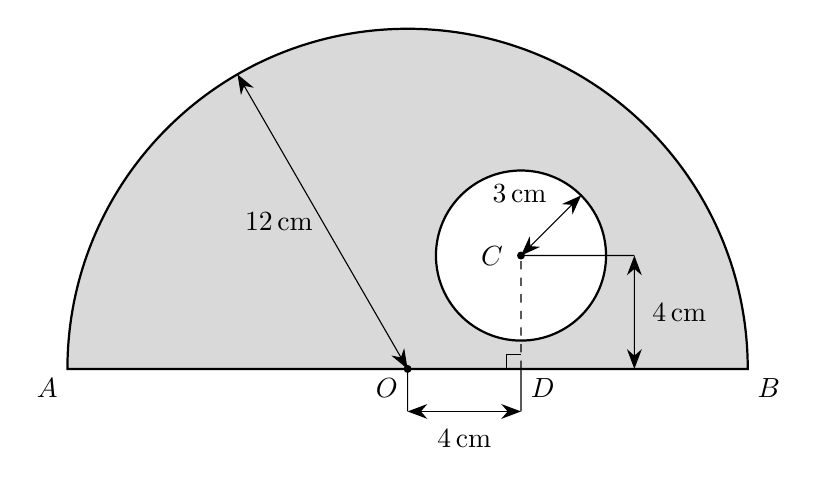
\begin{tikzpicture}[scale=0.36]
\def\rad{12}
\def\holeRad{3}
\def\offsetX{4}
\def\offsetY{4}
\def\markSize{0.5}
\def\dimDrop{1.5}
\def\dimShift{4}
\coordinate (O) at (0,0);
\coordinate (A) at (-\rad,0);
\coordinate (B) at (\rad,0);
\coordinate (D) at (\offsetX,0);
\coordinate (C) at ($(D)+(0,\offsetY)$);
\coordinate (P) at (120:\rad);
\coordinate (Q) at ($(C)+(45:\holeRad)$);
\coordinate (Od) at ($(O)+(0,-\dimDrop)$);
\coordinate (Dd) at ($(D)+(0,-\dimDrop)$);
\coordinate (Dv) at ($(D)+(\dimShift,0)$);
\coordinate (Cv) at ($(C)+(\dimShift,0)$);
\path[fill=gray!30,even odd rule] (A) arc[start angle=180,end angle=0,radius=\rad] -- cycle (C) circle (\holeRad);
\draw[thick,black] (A) arc[start angle=180,end angle=0,radius=\rad] -- cycle;
\draw[thick,black] (C) circle (\holeRad);
\draw[dashed,black] (D) -- (C);
\draw[thin,black] (O)--(Od) (D)--(Dd) (D)--(Dv) (C)--(Cv);
\draw[{Stealth[length=2.5mm]}-{Stealth[length=2.5mm]},black] (Od)--(Dd) node[midway,below=3pt] {$4\,\mathrm{cm}$};
\draw[{Stealth[length=2.5mm]}-{Stealth[length=2.5mm]},black] (Dv)--(Cv) node[midway,right=3pt] {$4\,\mathrm{cm}$};
\draw[black] ($(D)+(-\markSize,0)$) -- ($(D)+(-\markSize,\markSize)$) -- ($(D)+(0,\markSize)$);
\draw[{Stealth[length=2.5mm]}-{Stealth[length=2.5mm]},black] (O) -- (P) node[midway,left] {$12\,\mathrm{cm}$};
\draw[{Stealth[length=2.5mm]}-{Stealth[length=2.5mm]},black] (C) -- (Q) node[pos=0.65,above left=2pt] {$3\,\mathrm{cm}$};
\foreach \p in {O,C} {\fill[black] (\p) circle (4pt);}
\node[below left] at (A) {$A$};
\node[below right] at (B) {$B$};
\node[below left] at (O) {$O$};
\node[below right] at (D) {$D$};
\node[left=3pt] at (C) {$C$};
\end{tikzpicture}
\end{figure}


A uniform semicircular lamina has radius $12\,\mathrm{cm}$ and diameter $AB$, with midpoint $O$. \\
A circular hole of radius $3\,\mathrm{cm}$ is cut from the lamina. \\
Its centre $C$ is $4\,\mathrm{cm}$ above a point $D$ on $OB$, where $OD=4\,\mathrm{cm}$ and $CD$ is perpendicular to $AB$, as shown in the diagram above. \\

The remaining lamina is freely suspended from $B$ and hangs in equilibrium. \\

Determine the acute angle that $AB$ makes with the vertical, giving your answer to the nearest $0.1^\circ$. \\

You may use the result that the centre of mass of a uniform semicircular lamina of radius $r$ is on its axis of symmetry at a distance $\frac{4r}{3\pi}$ from its diameter. \marks{9} \\

\newpage

% ---- Question 2 ----
\questionitem
% [Source: _QBT__Centre_of_Mass_of_Circular_Laminae, Q2]

\begin{figure}[H]
    \centering
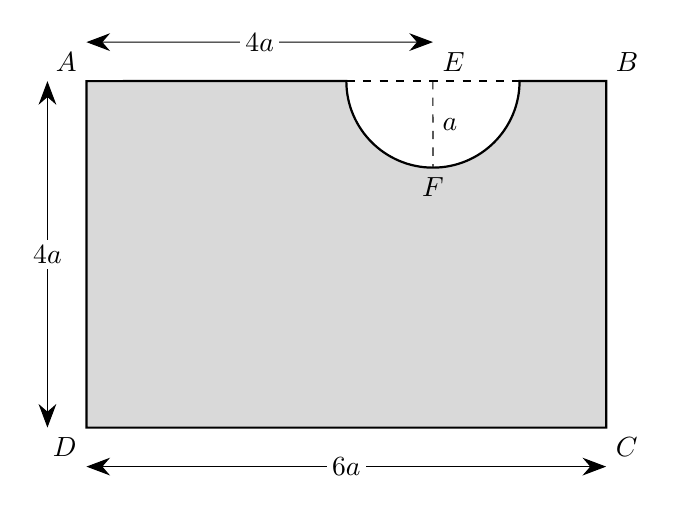
\begin{tikzpicture}[scale=1.1]
\def\a{1}
\def\dimoff{0.45}
\coordinate (D) at (0,0);
\coordinate (A) at ($(D)+(0,4*\a)$);
\coordinate (B) at ($(A)+(6*\a,0)$);
\coordinate (C) at ($(D)+(6*\a,0)$);
\coordinate (E) at ($(A)+(4*\a,0)$);
\coordinate (F) at ($(E)+(0,-\a)$);
\coordinate (L) at ($(E)+(-\a,0)$);
\coordinate (R) at ($(E)+(\a,0)$);
\fill[gray!30] (A) -- (L) arc[start angle=180,end angle=360,radius=\a] -- (B) -- (C) -- (D) -- cycle;
\draw[thick,black] (A) -- (L) arc[start angle=180,end angle=360,radius=\a] -- (B) -- (C) -- (D) -- cycle;
\draw[dashed,black] (L) -- (R);
\draw[dashed,black] (E) -- (F) node[midway,right] {$a$};
\draw[{Stealth[length=3mm]}-{Stealth[length=3mm]}] ($(D)+(0,-\dimoff)$) -- ($(C)+(0,-\dimoff)$) node[midway,fill=white,inner sep=2pt] {$6a$};
\draw[{Stealth[length=3mm]}-{Stealth[length=3mm]}] ($(D)+(-\dimoff,0)$) -- ($(A)+(-\dimoff,0)$) node[midway,fill=white,inner sep=2pt] {$4a$};
\draw[{Stealth[length=3mm]}-{Stealth[length=3mm]}] ($(A)+(0,\dimoff)$) -- ($(E)+(0,\dimoff)$) node[midway,fill=white,inner sep=2pt] {$4a$};
\node[above left] at (A) {$A$};
\node[above right] at (B) {$B$};
\node[below right] at (C) {$C$};
\node[below left] at (D) {$D$};
\node[above right] at (E) {$E$};
\node[below] at (F) {$F$};
\end{tikzpicture}
\end{figure}


A uniform rectangular lamina $ABCD$ has $AB=6a$ and $AD=4a$, where $a>0$. \\
A semicircular notch of radius $a$ is cut from the edge $AB$. \\
The centre $E$ of the semicircle lies on $AB$, with $AE=4a$, and the semicircle lies inside the rectangle, as shown in the diagram above. \\

You may use the result that the centre of mass of a uniform semicircular lamina of radius $r$ is a distance $\frac{4r}{3\pi}$ from its diameter. \\
\begin{enumerate}[label=\textbf{(\alph*)}]
\item
\begin{enumerate}[label=(\roman*)]
\item Show that the perpendicular distance of the centre of mass of the remaining lamina from $AD$ is
\[
\dfrac{4(36-\pi)}{48-\pi}a
\]
\item The remaining lamina is freely suspended from $A$ and hangs in equilibrium. Calculate the acute angle that $AB$ makes with the downward vertical, giving your answer to the nearest $0.1^\circ$.
\end{enumerate}
\end{enumerate}
\marks[-10pt]{9}

\newpage

% ---- Question 3 ----
\questionitem
% [Source: _QBT__Centre_of_Mass_of_Circular_Laminae, Q3]

\begin{figure}[H]
    \centering
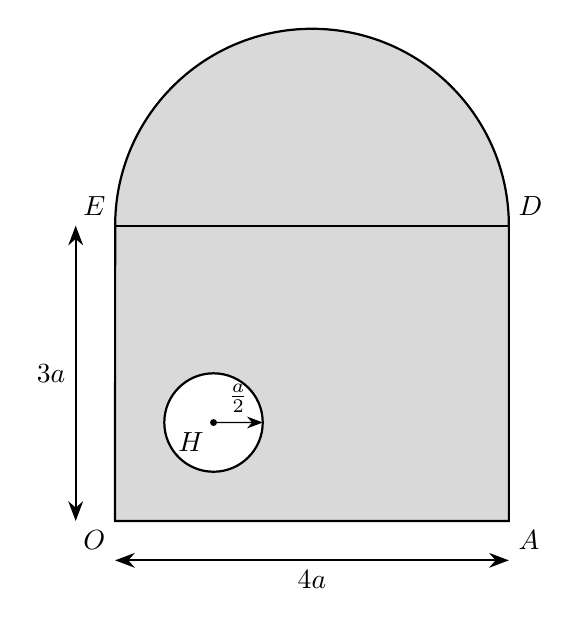
\begin{tikzpicture}[scale=1.25]
\def\a{1}
\def\width{4*\a}
\def\height{3*\a}
\def\semirad{2*\a}
\def\holerad{0.5*\a}
\def\dimoff{0.4*\a}
\coordinate (O) at (0,0);
\coordinate (A) at (\width,0);
\coordinate (D) at (\width,\height);
\coordinate (E) at (0,\height);
\coordinate (H) at (\a,\a);
\coordinate (R) at ($(H)+(0:\holerad)$);
\path[fill=gray!30,even odd rule] (O) -- (A) -- (D) arc[start angle=0,end angle=180,radius=\semirad] -- cycle (H) circle (\holerad);
\draw[thick,black] (O) -- (A) -- (D) arc[start angle=0,end angle=180,radius=\semirad] -- cycle;
\draw[thick,black] (E) -- (D);
\draw[thick,black] (H) circle (\holerad);
\draw[-{Stealth[length=2mm]},black] (H) -- (R) node[midway,above] {$\frac{a}{2}$};
\fill[black] (H) circle (1pt);
\node[below left] at (H) {$H$};
\node[below left] at (O) {$O$};
\node[below right] at (A) {$A$};
\node[above right] at (D) {$D$};
\node[above left] at (E) {$E$};
\draw[{Stealth[length=2.5mm]}-{Stealth[length=2.5mm]},thick] ($(O)+(0,-\dimoff)$) -- node[midway,below] {$4a$} ($(A)+(0,-\dimoff)$);
\draw[{Stealth[length=2.5mm]}-{Stealth[length=2.5mm]},thick] ($(O)+(-\dimoff,0)$) -- node[midway,left] {$3a$} ($(E)+(-\dimoff,0)$);
\end{tikzpicture}
\end{figure}


A uniform lamina is made by joining a rectangle $OADE$ to a semicircle along its diameter $ED$, and then removing a circular disc from the rectangular portion, as shown in the diagram above. \\

The rectangle has $OA=4a$ and $OE=3a$, where $a>0$. \\
The removed disc has radius $\frac{a}{2}$ and centre $H$, which is a distance $a$ from each of the sides $OE$ and $OA$. \\

You may use the result that the centre of mass of a uniform semicircular lamina of radius $r$ is a distance $\frac{4r}{3\pi}$ from its diameter. \\
\begin{enumerate}[label=\textbf{(\alph*)}]
\item Find, in terms of $a$ and $\pi$, the distance of the centre of mass of the remaining lamina from
\begin{enumerate}[label=(\roman*)]
\item $OE$,
\item $OA$.
\end{enumerate}
\marks[-10pt]{6}
\end{enumerate}
The remaining lamina is freely suspended from $A$ and hangs in equilibrium. \\
The angle between $AO$ and the downward vertical is $\alpha$. \\
\begin{enumerate}[label=\textbf{(\alph*)}, resume]
\item Find the exact value of $\tan\alpha$. \marks{2} \\
\end{enumerate}

\newpage

% ---- Question 4 ----
\questionitem
% [Source: _QBT__Centre_of_Mass_of_Circular_Laminae, Q4]

\begin{figure}[H]
    \centering
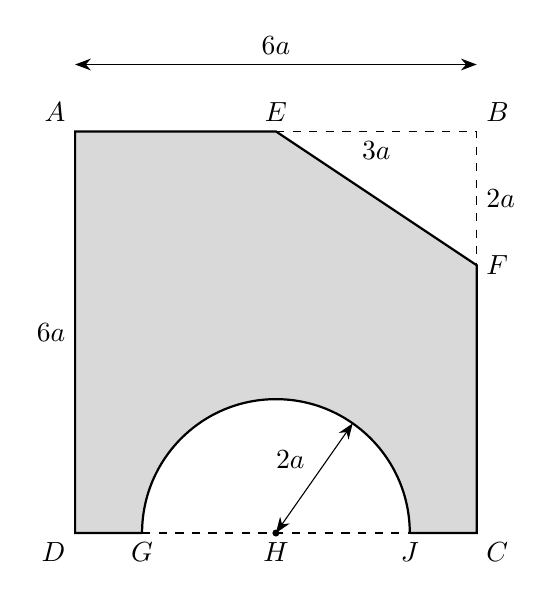
\begin{tikzpicture}[scale=0.85]
\def\s{6}
\def\leg{3}
\def\drop{2}
\def\rad{2}
\def\dimoff{1}
\def\radiusang{55}
\coordinate (D) at (0,0);
\coordinate (A) at (0,\s);
\coordinate (B) at (\s,\s);
\coordinate (C) at (\s,0);
\coordinate (E) at ({\s-\leg},\s);
\coordinate (F) at (\s,{\s-\drop});
\coordinate (H) at ({\s/2},0);
\coordinate (G) at ($(H)+(-\rad,0)$);
\coordinate (J) at ($(H)+(\rad,0)$);
\coordinate (R) at ($(H)+(\radiusang:\rad)$);
\fill[gray!30] (A)--(E)--(F)--(C)--(D)--cycle;
\fill[white] (G) arc[start angle=180,end angle=0,radius=\rad] -- cycle;
\draw[thick,black] (G)--(D)--(A)--(E)--(F)--(C)--(J);
\draw[thick,black] (G) arc[start angle=180,end angle=0,radius=\rad];
\draw[dashed,black] (E)--(B)--(F);
\draw[dashed,black] (G)--(J);
\draw[{Stealth[length=2mm]}-{Stealth[length=2mm]}] ($(A)+(0,\dimoff)$)--($(B)+(0,\dimoff)$) node[midway,above] {$6a$};
\path (A)--(D) node[midway,left] {$6a$};
\path (E)--(B) node[midway,below] {$3a$};
\path (B)--(F) node[midway,right] {$2a$};
\draw[{Stealth[length=2mm]}-{Stealth[length=2mm]}] (H)--(R) node[midway,above left] {$2a$};
\fill[black] (H) circle (1.5pt);
\foreach \p/\pos in {A/above left,B/above right,C/below right,D/below left,E/above,F/right,G/below,H/below,J/below} {
  \node[\pos] at (\p) {$\p$};
}
\end{tikzpicture}
\end{figure}


A uniform square lamina $ABCD$ has side $6a$. \\
A template $T$, shown shaded in the diagram above, is made by removing two portions of the lamina. \\

The first portion is the right-angled triangle $EBF$, where $E$ lies on $AB$, $F$ lies on $BC$, $EB=3a$ and $BF=2a$. \\

The second portion is a semicircle of radius $2a$. \\
Its centre $H$ is the midpoint of $DC$, its diameter lies on $DC$, and the semicircle lies inside the square. \\

\begin{enumerate}[label=\textbf{(\alph*)}]
\item Find the distances of the centre of mass of $T$ from $AD$ and from $DC$, giving both answers exactly in terms of $a$ and $\pi$. \marks{6} \\
\end{enumerate}
The template is now freely suspended from $A$ and hangs in equilibrium in a vertical plane. \\
\begin{enumerate}[label=\textbf{(\alph*)}, resume]
\item Find the acute angle between $AD$ and the vertical, giving your answer to the nearest $0.1^\circ$. \marks{3} \\
\end{enumerate}

\newpage

% ---- Question 5 ----
\questionitem
% [Source: _QBT__Centre_of_Mass_of_Circular_Laminae, Q5]

\begin{figure}[H]
    \centering
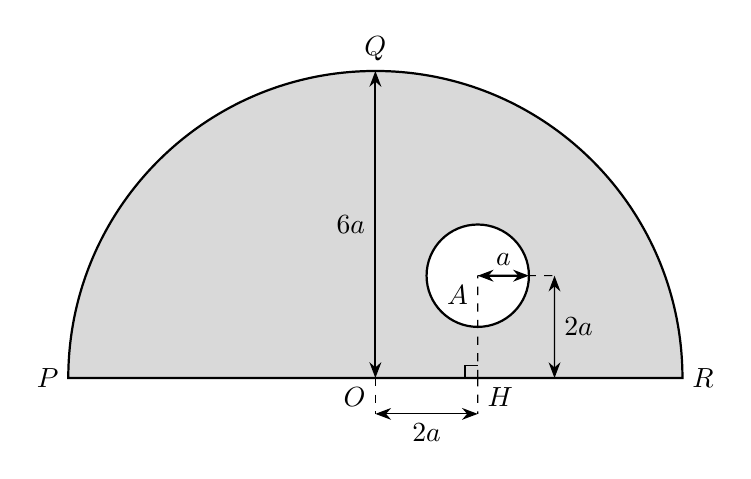
\begin{tikzpicture}[scale=0.65]
\def\a{1}
\def\rad{6*\a}
\def\holerad{\a}
\def\offset{2*\a}
\def\dimdrop{0.7*\a}
\def\dimshift{1.5*\a}
\def\marksize{0.25*\a}
\coordinate (O) at (0,0);
\coordinate (P) at (180:\rad);
\coordinate (Q) at (90:\rad);
\coordinate (R) at (0:\rad);
\coordinate (H) at (\offset,0);
\coordinate (A) at ($(H)+(0,\offset)$);
\coordinate (Ar) at ($(A)+(\holerad,0)$);
\coordinate (Od) at ($(O)+(0,-\dimdrop)$);
\coordinate (Hd) at ($(H)+(0,-\dimdrop)$);
\coordinate (Hv) at ($(H)+(\dimshift,0)$);
\coordinate (Av) at ($(A)+(\dimshift,0)$);
\fill[gray!30] (P) arc[start angle=180,end angle=0,radius=\rad] -- cycle;
\fill[white] (A) circle (\holerad);
\draw[thick,black] (P) arc[start angle=180,end angle=0,radius=\rad] -- cycle;
\draw[thick,black] (A) circle (\holerad);
\draw[dashed,black] (H) -- (A);
\draw[{Stealth[length=2mm]}-{Stealth[length=2mm]},thick,black] (O) -- (Q) node[midway,left] {$6a$};
\draw[{Stealth[length=2mm]}-{Stealth[length=2mm]},thick,black] (A) -- (Ar) node[midway,above] {$a$};
\foreach \point/\end in {O/Od,H/Hd,H/Hv,A/Av} {
  \draw[dashed,black] (\point) -- (\end);
}
\draw[{Stealth[length=2mm]}-{Stealth[length=2mm]},black] (Od) -- (Hd) node[midway,below] {$2a$};
\draw[{Stealth[length=2mm]}-{Stealth[length=2mm]},black] (Hv) -- (Av) node[midway,right] {$2a$};
\draw[black] ($(H)+(-\marksize,0)$) -- ($(H)+(-\marksize,\marksize)$) -- ($(H)+(0,\marksize)$);
\node[left] at (P) {$P$};
\node[above] at (Q) {$Q$};
\node[right] at (R) {$R$};
\node[below left] at (O) {$O$};
\node[below right] at (H) {$H$};
\node[below left] at (A) {$A$};
\end{tikzpicture}
\end{figure}


A uniform semicircular lamina has centre $O$, radius $6a$ and diameter $PR$. \\
A circular disc of radius $a$ is removed to form the lamina $L$ shown shaded in the diagram above. \\
The centre of the removed disc is $A$. \\
The point $H$ lies on $OR$, with $OH=2a$, $HA=2a$ and $HA$ perpendicular to $PR$. \\

Take $O$ as the origin, with the positive $x$-axis directed towards $R$ and the positive $y$-axis directed towards $Q$. \\
\begin{enumerate}[label=\textbf{(\alph*)}]
\item Find the exact coordinates of the centre of mass of $L$. \marks{6} \\
\end{enumerate}
The mass of $L$ is $M$. \\
A particle of mass $kM$ is attached at $P$. \\
The system is freely suspended from $R$ and hangs in equilibrium, with $P$ below $R$ and the diameter $PR$ making an acute angle of $\arctan\left(\frac{1}{6}\right)$ with the downward vertical through $R$. \\
\begin{enumerate}[label=\textbf{(\alph*)}, resume]
\item Find the exact value of $k$ and the magnitude of the supporting force at $R$ in terms of $M$ and $g$. \marks{6} \\
\end{enumerate}

\newpage

% ---- Question 6 ----
\questionitem
% [Source: _QBT__Centre_of_Mass_of_Circular_Laminae, Q6]

\begin{figure}[H]
    \centering
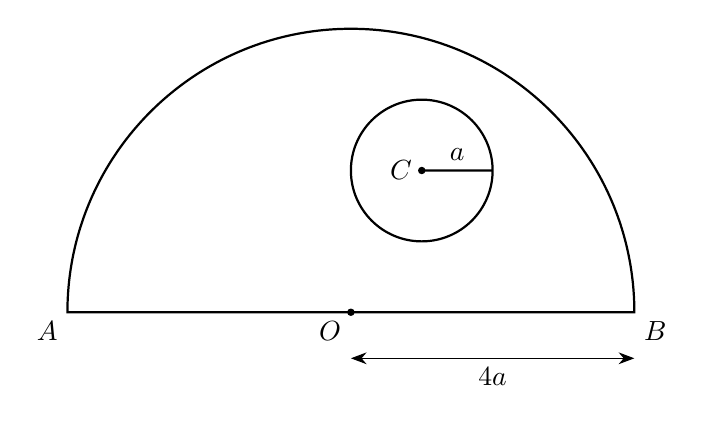
\begin{tikzpicture}[scale=0.9]
\def\rad{4}
\def\hole{1}
\def\cx{1}
\def\cy{2}
\def\dimdrop{0.65}
\coordinate (O) at (0,0);
\coordinate (A) at (-\rad,0);
\coordinate (B) at (\rad,0);
\coordinate (C) at (\cx,\cy);
\coordinate (E) at ($(C)+(\hole,0)$);
\draw[thick,black] (B) arc[start angle=0,end angle=180,radius=\rad] -- cycle;
\draw[thick,black] (C) circle (\hole);
\draw[thick,black] (C)--(E) node[midway,above] {$a$};
\foreach \p in {O,C} {\fill[black] (\p) circle (1.5pt);}
\node[below left] at (A) {$A$};
\node[below right] at (B) {$B$};
\node[below left] at (O) {$O$};
\node[left] at (C) {$C$};
\coordinate (Om) at ($(O)+(0,-\dimdrop)$);
\coordinate (Bm) at ($(B)+(0,-\dimdrop)$);
\draw[{Stealth[length=2mm]}-{Stealth[length=2mm]}] (Om)--(Bm) node[midway,below] {$4a$};
\end{tikzpicture}
\end{figure}


A uniform semicircular lamina has radius $4a$ and diameter $AB$, whose midpoint is $O$. \\
A circular hole of radius $a$ is cut from the lamina. \\
In the orientation shown above, take $O$ as the origin, the positive $x$-direction along $OB$ and the positive $y$-direction perpendicular to $AB$ towards the semicircular arc. \\
The centre $C$ of the hole has coordinates $(a,2a)$. \\
\begin{enumerate}[label=\textbf{(\alph*)}]
\item Show that the centre of mass $G$ of the remaining lamina has coordinates
\[
\left(-\dfrac{a}{7},\ \dfrac{(128-6\pi)a}{21\pi}\right)
\] \marks[-30pt]{6}
\end{enumerate}
The remaining lamina has mass $7\,\mathrm{kg}$. \\
It is freely pivoted at $A$ and turned so that $AB$ is vertical, with $A$ above $B$ and the semicircular arc to the right of $AB$, as shown in the diagram below. \\
A light string attached to $B$ holds the lamina in equilibrium. \\
The string lies in the plane of the lamina and makes an angle of $30^\circ$ below the horizontal. \\
\begin{figure}[H]
    \centering
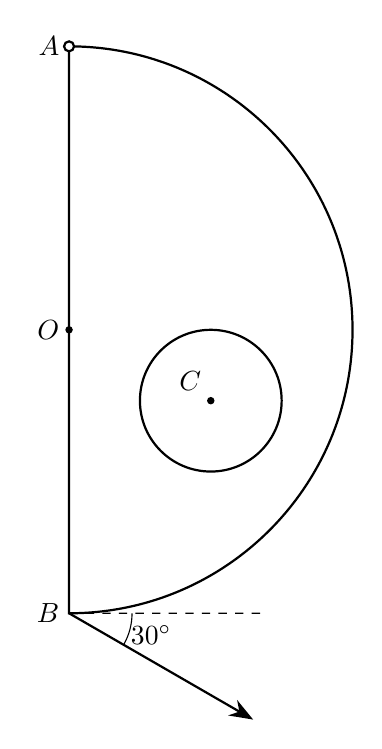
\begin{tikzpicture}[scale=0.9]
\def\rad{4}
\def\hole{1}
\def\cx{1}
\def\cy{2}
\def\stringlen{3}
\def\horizlen{2.8}
\def\ang{30}
\coordinate (O) at (0,0);
\coordinate (A) at (0,\rad);
\coordinate (B) at (0,-\rad);
\coordinate (C) at (\cy,-\cx);
\coordinate (H) at ($(B)+(\horizlen,0)$);
\coordinate (S) at ($(B)+(-\ang:\stringlen)$);
\draw[thick,black] (B) arc[start angle=-90,end angle=90,radius=\rad] -- cycle;
\draw[thick,black] (C) circle (\hole);
\draw[dashed,black] (B)--(H);
\draw[-{Stealth[length=3mm]},thick,black] (B)--(S);
\pic["$30^\circ$",draw,angle radius=8mm,angle eccentricity=1.35] {angle=S--B--H};
\foreach \p in {O,C} {\fill[black] (\p) circle (1.5pt);}
\draw[thick,fill=white] (A) circle (2pt);
\foreach \p in {A,B,O} {\node[left] at (\p) {$\p$};}
\node[above left] at (C) {$C$};
\end{tikzpicture}
\end{figure}


\begin{enumerate}[label=\textbf{(\alph*)}, resume]
\item Calculate the tension in the string. \marks{3} \\
\item Find the magnitude of the force exerted on the lamina by the pivot at $A$ and the angle this force makes with the upward vertical, stating on which side of the vertical it acts. \marks{5} \\
\end{enumerate}

\newpage

% ---- Question 7 ----
\questionitem
% [Source: _QBT__Centre_of_Mass_of_Circular_Laminae, Q7]

A uniform lamina consists of a rectangle $ABCD$ together with a semicircular tab $EFG$ attached externally along its diameter $EG$, as shown in the diagram below.
The two components have the same mass per unit area.
The points $E$ and $G$ lie on $BC$, and $O$ is the midpoint of $EG$.

The dimensions are $AB=6\,\mathrm{cm}$, $BC=18\,\mathrm{cm}$ and $BE=3\,\mathrm{cm}$.
The semicircular tab has radius $3\,\mathrm{cm}$.

\begin{figure}[H]
    \centering
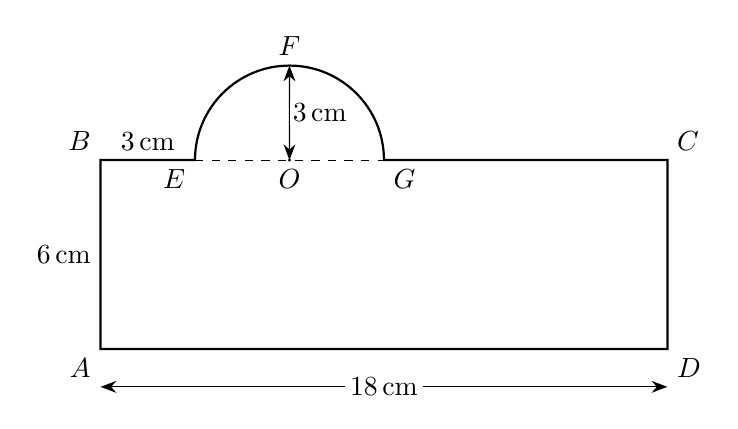
\begin{tikzpicture}[scale=0.4]
\def\W{18}\def\H{6}\def\ox{6}\def\rad{3}\def\dimdrop{1.2}
\coordinate (A) at (0,0);
\coordinate (B) at (0,\H);
\coordinate (C) at (\W,\H);
\coordinate (D) at (\W,0);
\coordinate (O) at (\ox,\H);
\coordinate (E) at ($(O)+(-\rad,0)$);
\coordinate (F) at ($(O)+(0,\rad)$);
\coordinate (G) at ($(O)+(\rad,0)$);
\draw[thick,black] (A)--(B)--(E) arc[start angle=180,end angle=0,radius=\rad] --(C)--(D)--cycle;
\draw[dashed] (E)--(G);
\foreach \p/\pos in {A/below left,B/above left,C/above right,D/below right,E/below left,F/above,G/below right} {\node[\pos] at (\p) {$\p$};}
\fill (O) circle (1.5pt);
\node[below] at (O) {$O$};
\path (A)--(B) node[midway,left] {$6\,\mathrm{cm}$};
\draw[{Stealth[length=2mm]}-{Stealth[length=2mm]}] ($(A)+(0,-\dimdrop)$)--($(D)+(0,-\dimdrop)$) node[midway,fill=white,inner sep=2pt] {$18\,\mathrm{cm}$};
\path (B)--(E) node[midway,above] {$3\,\mathrm{cm}$};
\draw[{Stealth[length=2mm]}-{Stealth[length=2mm]}] (O)--(F) node[midway,right,fill=white,inner sep=1pt] {$3\,\mathrm{cm}$};
\end{tikzpicture}
\end{figure}


\begin{enumerate}[label=\textbf{(\alph*)}]
\item Consider the semicircular tab $EFG$ on its own. Using the standard centre-of-mass result for a uniform semicircular lamina, show that its centre of mass is $1.27\,\mathrm{cm}$ from the diameter $EG$, correct to $3$ significant figures. State the exact distance. \marks{2}

\item For the complete lamina, find
\begin{enumerate}[label=(\roman*)]
\item the distance from $AB$ to its centre of mass, giving your answer exactly, \marks{4}
\item the distance from $AD$ to its centre of mass, giving your answer exactly. \marks{3}
\end{enumerate}

\item The complete lamina has weight $24\,\mathrm{N}$ and is smoothly pivoted at $A$.
A wire attached at $C$ supports it in equilibrium.
The wire pulls upwards and to the left at $30^\circ$ above the horizontal, and its tension is $10\,\mathrm{N}$.

The side $AD$ makes an angle $\theta$ above the horizontal, where $0^\circ<\theta<45^\circ$, as shown in the diagram below.

\begin{figure}[H]
    \centering
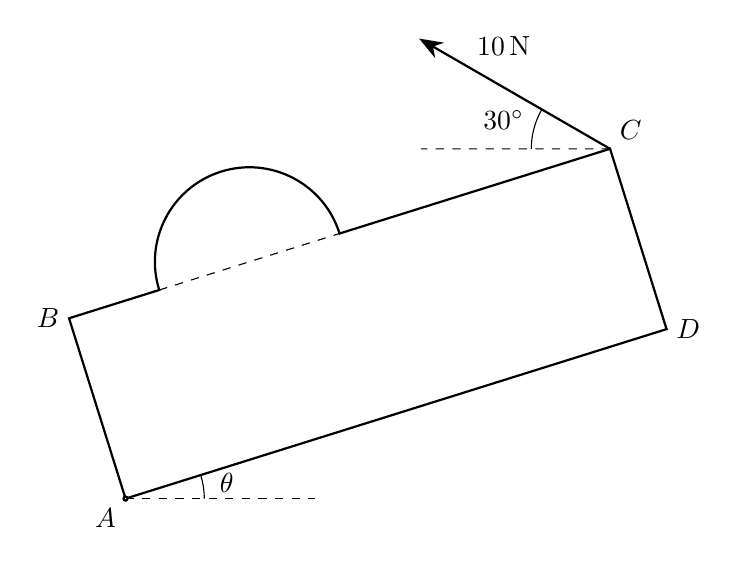
\begin{tikzpicture}[scale=0.4]
\def\W{18}\def\H{6}\def\ox{6}\def\rad{3}\def\wirelen{7}\def\reflen{6}\def\wireang{150}
\pgfmathsetmacro{\area}{\W*\H+pi*\rad^2/2}
\pgfmathsetmacro{\xbar}{(\W*\H*\W/2+(pi*\rad^2/2)*\ox)/\area}
\pgfmathsetmacro{\ybar}{(\W*\H*\H/2+(pi*\rad^2/2)*(\H+4*\rad/(3*pi)))/\area}
\pgfmathsetmacro{\ang}{atan((24*\xbar-10*(\W/2+sqrt(3)*\H/2))/(10*(sqrt(3)*\W/2-\H/2)+24*\ybar))}
\coordinate (A) at (0,0);
\coordinate (X) at (\reflen,0);
\begin{scope}[rotate=\ang]
\coordinate (B) at (0,\H);
\coordinate (C) at (\W,\H);
\coordinate (D) at (\W,0);
\coordinate (O) at (\ox,\H);
\coordinate (E) at ($(O)+(-\rad,0)$);
\coordinate (G) at ($(O)+(\rad,0)$);
\draw[thick,black] (A)--(B)--(E) arc[start angle=180,end angle=0,radius=\rad] --(C)--(D)--cycle;
\draw[dashed] (E)--(G);
\end{scope}
\coordinate (L) at ($(C)+(-\reflen,0)$);
\coordinate (S) at ($(C)+(\wireang:\wirelen)$);
\draw[dashed] (A)--(X);
\draw[dashed] (C)--(L);
\draw[-{Stealth[length=3mm]},thick,black] (C)--(S) node[pos=0.75,above right] {$10\,\mathrm{N}$};
\pic["$\theta$",draw,angle radius=10mm,angle eccentricity=1.3] {angle=X--A--D};
\pic["$30^\circ$",draw,angle radius=10mm,angle eccentricity=1.4] {angle=S--C--L};
\draw[thick,fill=white] (A) circle (1.8pt);
\node[below left] at (A) {$A$};
\node[left] at (B) {$B$};
\node[above right] at (C) {$C$};
\node[right] at (D) {$D$};
\end{tikzpicture}
\end{figure}


Calculate $\theta$, giving your answer to $3$ significant figures. \marks{6}
\end{enumerate}

\end{enumerate}
\end{document}
